\usetikzlibrary{positioning, chains, shapes.geometric, fit, shapes, arrows.meta, calc, backgrounds}

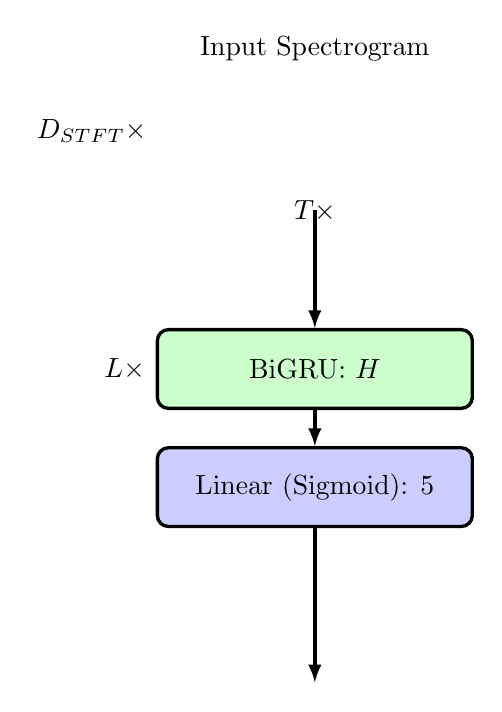
\begin{tikzpicture}[
    >=LaTeX, 
    very thick,
    arrow/.style={
        -latex,
        very thick,
        rounded corners=0.2cm
    },
    ]


%\draw[transform canvas={xscale=2}, step=0.125cm, ultra thin] (-1, 0.25) grid (1, 1.75);
%\draw[thick] (-2, 0.25) -- (2, 0.25) -- (2, 1.75) -- (-2, 1.75) -- cycle;
\node[anchor=south] at (0, 1.75) {Input Spectrogram};
\node[anchor=east] at (-2, 1) {$D_\text{STFT}\times$};
\node[anchor=north] at (0, 0.25) {$T\times$};

\draw[arrow] (0, 0) -- (0, -1.5) node[rectangle, 
rounded corners, 
draw, 
anchor=north, 
label=west:$L\times$,
fill=green!20,
minimum height=1cm,
minimum width=4cm
] (a) {BiGRU: $H$};

\draw[arrow] (a) -- (0, -3) node[rectangle, 
rounded corners, 
draw, 
anchor=north, 
fill=blue!20,
minimum height=1cm,
minimum width=4cm
] (b) {Linear (Sigmoid): $5$};

\draw[arrow] (b) -- (0, -6);

\end{tikzpicture}